\section{Tipagem dinâmica e estática}

\begin{frame}{Tipagem dinâmica e estática}
\framesubtitle{Escolha de design}
\begin{itemize}
    \item No paradigma orientado a objetos, as linguagens possuem uma escolha com relação à tipagem: dinâmica ou estática
    \item Equilíbrio entre o custo de execução e de compilação
    \item Algumas linguagens de orientação a objetos realizam vínculo estático ou dinâmico a depender de algumas condições específicas
\end{itemize} 
\end{frame}

\begin{frame}[fragile]{Tipagem dinâmica}
\begin{itemize}
    \item Muitas vezes, chamadas internas a métodos implementados por subclasses possuem uma informação incompleta
    \item Em Java, por exemplo, há diversas implementações do método add em classes diferentes.
\end{itemize}
\begin{verbatim}
        this.add(elemento);
\end{verbatim}
\end{frame}

\begin{frame}[fragile]{Tipagem dinâmica}
\begin{itemize}
    \item Muito comum para situações de polimorfismo
    \item Uma referência pode apontar para objetos de classes distintas
    \item O sistema precisa determinar, em tempo de execução, a qual classe um método se refere, visto que há ambiguidade
    \item Provê facilidade no desenvolvimento e manutenção dos objetos da aplicação
\end{itemize}
\end{frame}


\begin{frame}[fragile]{Tipagem estática}
\begin{itemize}
    \item Muitas vezes um custo de execução pode ser convertido em compilação
    \item A informação completa ou restrição do contexto permite essa conversão
    \item Em Java, por exemplo, quando não há dúvidas da origem de uma chamada de um método, o compilador armazena as informações dos métodos e classes utilizadas
\end{itemize}
\begin{verbatim}
        colecao.addAll(outraColecao);
\end{verbatim}
\begin{itemize}
    \item A classe precisa implementar AbstractCollection, e portanto o método addAll deve ser definido como static ou final
\end{itemize}
\end{frame}

\section{Exemplos de linguagens}

\subsection{Smalltalk}

\begin{frame}{Smalltalk}
\framesubtitle{Histórico}
    \begin{itemize}
        \item Teve inicio com um projeto de pesquisa na Xerox Corporation's Palto Alto Research Center em 1970
        \item Foi continuado por Adele Goldberg e Daniel Ingalls
        \item Influência de Simula e Lisp
        \item Foi inovadora para a divisória criada para interfaces gráficas.
        \item Ambiente de desenvolvimento completo, com sistemas de janelas, menus e cursor
    \end{itemize}
\end{frame}

\begin{frame}{Smalltalk}
\framesubtitle{Design}
    \begin{itemize}
        \item Puramente orientada a objetos (até constantes)
        \item Mensagens e Objetos de dados
        \item Objetos possuem características e comportamentos
    \end{itemize}
\end{frame}

\begin{frame}[fragile]{Smalltalk}
\framesubtitle{Design}
    \begin{itemize}
        \item Características são atributos de uma classe ou instância
        \item Comportamentos são ações a serem reproduzidas por métodos
        \item Métodos podem enviar outras mensagens e podem devolver objetos
        \item Mensagens podem ser unárias ou até mesmo incluir parâmetros
    \end{itemize}
\begin{verbatim}
        Set new includes: 'Hello'
        (Array new: 10) at: 1 put: 66
\end{verbatim}
\end{frame}

\begin{frame}{Smalltalk}
    \begin{figure}
	\centering
	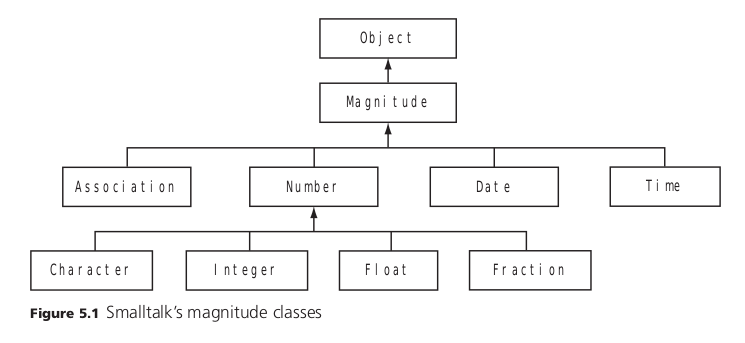
\includegraphics[width=0.8\linewidth]{img/magnitude}
	\caption{Hierarquia de classes de magnitude \cite{louden2012}}
	\label{fig:herancadiamante}
\end{figure}
\end{frame}
